\section{Radiative Transfer Calculations}
%========================================
\label{sec:rt}

Monochromatic radiative transfer (RT) calculations were done at the various tabulated ATMS SRF frequencies using MonoRTM \cite{Payne_2008,Clough_2005} and the ECMWF83 profile set \cite{Matricardi_ECMWF564,ECMWF_profile_set2}. The RT calculations were done for a simple surface emissivity and reflectivity of $\epsilon_s=0.6$ and $r_s=0.4$ respectively. The subsequent spectra were then convolved with the digitized SRFs using a numerical integration routine.

The temperature and water vapour from the ECMWF83 set are shown in figure \ref{fig:ECMWF83.AtmProfile} to provide an indication of the range of inputs.

\begin{figure}[htp]
  \centering
  \includegraphics[scale=1]{graphics/atmprofile/ECMWF83.AtmProfile.eps}
  \caption{The temperature and water vapour profiles from the ECMWF83 profile dataset used in the radiative transfer calculations.}
  \label{fig:ECMWF83.AtmProfile}
\end{figure}

The results for the different SRFs are presented here as brightness temperature differences from the nominal SRF result; that is,
\begin{equation}
  \Delta T_B = T_{B,Measured} - T_{B,ref} 
\end{equation}
The $\Delta T_B$ values are displayed as a function of $T_{B,ref}$. Only the results for those channels for which there are large differences will be discussed here. Results for all the channels are shown in Appendices \ref{app:Tset}, \ref{app:Vset}, \ref{app:Rset} for the baseplate temperature, bias voltage, and spectral resolution comparison datasets respectively.

Since the reference for the brightness temperatures differences is the boxcar SRF, it should also be noted that these comparisons are intended to highlight the impact of the differences between the various digitized SRFs, not necessarily to indicate which is ``better''.


\subsection{$\Delta T_B$ for Variable Temperature SRFs}
%------------------------------------------------------
\label{sec:rt.Tset}
This section discusses the $\Delta T_B$ residual results for the variable baseplate temperature SRF datasets. Not all of the channel results will be covered here, just a selection of channels that highlights the SRF differences and explains the $\Delta T_B$ residuals. See appendix \ref{app:Tset} for plots of all the temperature dataset SRFs and appendix \ref{app:Tset_dtb_data_plots} for $\Delta T_B$ residuals for all channels.


\begin{figure}[H]
  \centering
    \includegraphics[scale=0.7]{graphics/dtb/Tset/atms_npp.Tset.dTb_stats.eps} 
  \caption{Statistics of the MonoRTM-derived ATMS channel brightness temperature residuals, using a surface emissivity and reflectivity of 0.6 and 0.4 respectively, for the low and high temperature SRF datasets compared to the nominal temperature SRF, for the nominal bias voltage.}
  \label{fig:Tset_dTb_stats}
\end{figure}



\subsubsection{Channel 1}
%........................
The Tset SRFs for channel 1 are shown in figure \ref{sec:rt.Tset_fig:atms_npp.Tset.ch1}(a). There is a significant difference in the shape of the -10\textdegree{}C SRF including a decrease in the SRF width on the low-frequency side. The variation in the shapes of the 20\textdegree{}C and 50\textdegree{}C SRF shapes follow each other relatively well, even if their magnitudes differ. Note also the variation of the brightness temperature spectrum across the SRF bandwidth is quite small, only $\sim$0.04K.

The effect of the SRF shape differences are somewhat evident in the $\Delta T_B$ residuals of figure \ref{sec:rt.Tset_fig:atms_npp.Tset.ch1}(b). Overall, the variation in residuals does not typically exceed $\pm$0.01K. The $\Delta T_B$ residuals for the similar 20\textdegree{}C and 50\textdegree{}C SRFs are themselves quite similar. The negative residuals are due to the SRFs being shifted slightly toward lower frequencies; and thus weight the cooler portion of the spectra in the band compared to the reference boxcar. The -10\textdegree{}C SRF $\Delta T_B$ residuals are about the same size of the other two but of opposite sign. This can be explained by the low frequency side of the -10\textdegree{}C SRF having a much lower magnitude, coupled with the shift of the low-frequency passband edge to a slightly higher frequency. The effect of these SRF differences would weight the right side of the SRF more, which corresponds to the warmer part of the spectrum.
\begin{figure}[H]
  \centering
  \hspace{-0.5cm}\textsf{\textbf{(a)} SRFs} \\
  \includegraphics[trim={90 0 10 20},clip,scale=0.6]{graphics/srf/Tset/lin/atms_npp-1.eps} \\
  \hspace{-0.5cm}\textsf{\textbf{(b)} $\Delta T_B$ $(\epsilon_s = 0.6)$} \\
  \includegraphics[trim={10 0 40 0},clip,scale=0.45]{graphics/dtb/Tset/atms_npp.ch1.dTb_T_PW_stats.eps} 
  \caption{ATMS channel 1 at nominal bias voltage. \textbf{(a)} SRF data for the three test temperatures (20\textdegree{}C is nominal). \textbf{(b)} Difference in the MonoRTM-derived brightness temperatures for -10 and 50\textdegree{}C compared to the nominal temperature, using a surface emissivity of 0.6 and the ECMWF83 profile set.}
  \label{sec:rt.Tset_fig:atms_npp.Tset.ch1}
\end{figure}


\subsubsection{Channel 2}
%........................
The Tset SRFs for channel 2 are shown in figure \ref{sec:rt.Tset_fig:atms_npp.Tset.ch2}(a). There are quite evident differences in the shapes of the SRFs across the band, as well as a significant shift (roughly 5\%) of all the SRFs to lower frequencies. For this window channel, the variation of the brightness temperature spectrum across the SRF bandwidth is again quite small, only $\sim$0.01K.

Even though the SRF shapes oscillate in-band, the overall effect will tend to average out. Coupled with the fact that this is a window channel, the $\Delta T_B$ residuals of figure \ref{sec:rt.Tset_fig:atms_npp.Tset.ch2}(b) are both similar for all the SRFs and small. The small positive bias in the residuals can be attributed to the overall SRF frequency shift which will emphasise the warmer regions of the in-band spectra.
\begin{figure}[H]
  \centering
  \begin{tabular}{c c c}
    \textsf{\textbf{(a)} SRFs} &
    \textsf{\textbf{(b)} $\Delta T_B$ $(\epsilon_s = 1.0)$} &
    \textsf{\textbf{(c)} $\Delta T_B$ $(\epsilon_s = 0.6)$} \\
    \includegraphics[bb=80 400 280 558,clip,scale=0.85]{graphics/srf/Tset/atms_npp.ch2.osrf.eps} &
    \includegraphics[bb=85 400 260 558,clip,scale=0.85]{graphics/dtb/Tset/e1.0_r0.0/atms_npp.ch2.dTb.eps} & 
    \includegraphics[bb=85 400 290 558,clip,scale=0.85]{graphics/dtb/Tset/e0.6_r0.4/atms_npp.ch2.dTb.eps} 
  \end{tabular} \\
  % the hand-crafted legend
  \setlength{\unitlength}{1cm}
  \begin{picture}(8.0,1.0)
    \thicklines
    \color{red}
    \put(0.0,0.5){\line(1,0){1}}
    \put(1.2,0.35){\sffamily \textbf{+}\quad -10\textdegree{}C}
    \color{green}
    \put(3.0,0.5){\line(1,0){1}}
    \put(4.2,0.35){\sffamily {\Large$\diamond$}\quad 20\textdegree{}C}
    \color{blue}
    \put(6.0,0.5){\line(1,0){1}}
    \put(7.2,0.35){\sffamily $\bigtriangleup$\quad 50\textdegree{}C}
  \end{picture}
  \caption{Channel 2 NPP ATMS \textbf{(a)} SRF data digitized from plots in the ATMS PFM Calibration Data Book\cite{ATMS_PFM_CalLog} with the corresponding boxcar response based on table \ref{tab:atms_fo_sb_and_df}. A representative brightness temperature spectrum is also shown. \textbf{(b)} Difference in the MonoRTM-derived brightness temperatures, using unity surface emissivity, as a function of the boxcar SRF $T_B$ for nominal bias voltage and three baseplate temperatures (-10, 20, and 50\textdegree{}C). \textbf{(c)} Same as (b), but for surface emissivity and reflectivity of 0.6 and 0.4 respectively. }
  \label{sec:rt.Tset_fig:atms_npp.Tset.ch2}
\end{figure}



\subsubsection{Channel 4}
%........................
The Tset SRFs for channel 4 are shown in figure \ref{sec:rt.Tset_fig:atms_npp.Tset.ch4}(a). The -10\textdegree{}C and 20\textdegree{}C SRFs are similar in shape but asymmetrical, weighting the higher frequencies and, thus, the cooler regions of the in-band spectra. Additionally, the -10\textdegree{}C SRF has a small shift to higher frequencies. The 50\textdegree{}C SRF is more symmetrical. For this channel, the variation of the brightness temperature spectrum across the SRF bandwidth is significant, around 2K.

The larger range of the in-band spectra for this channel, coupled with the SRF asymmetries mentioned above, produces relatively large $\Delta T_B$ residuals compared to a boxcar reference, up to 0.1K. The residuals in figure \ref{sec:rt.Tset_fig:atms_npp.Tset.ch4}(b) indicate the asymmetry of the -10\textdegree{}C and 20\textdegree{}C SRFs are the biggest factor, with the slight shift to higher frequencies inceasing the weight of the cooler portions of the in-band spectra for the -10\textdegree{}C SRF. The 50\textdegree{}C SRF residuals are quite small given the range of the in-band spectra - the small positive bias is likely due to a combination of SRF shape and the high frequency band edge occuring at slightly lower frequencies. 
\begin{figure}[H]
  \centering
  \begin{tabular}{c c c}
    \textsf{\textbf{(a)} SRFs} &
    \textsf{\textbf{(b)} $\Delta T_B$ $(\epsilon_s = 1.0)$} &
    \textsf{\textbf{(c)} $\Delta T_B$ $(\epsilon_s = 0.6)$} \\
    \includegraphics[bb=80 400 280 558,clip,scale=0.85]{graphics/srf/Tset/atms_npp.ch4.osrf.eps} &
    \includegraphics[bb=85 400 260 558,clip,scale=0.85]{graphics/dtb/Tset/e1.0_r0.0/atms_npp.ch4.dTb.eps} & 
    \includegraphics[bb=85 400 290 558,clip,scale=0.85]{graphics/dtb/Tset/e0.6_r0.4/atms_npp.ch4.dTb.eps} 
  \end{tabular} \\
  % the hand-crafted legend
  \setlength{\unitlength}{1cm}
  \begin{picture}(8.0,1.0)
    \thicklines
    \color{red}
    \put(0.0,0.5){\line(1,0){1}}
    \put(1.2,0.35){\sffamily \textbf{+}\quad -10\textdegree{}C}
    \color{green}
    \put(3.0,0.5){\line(1,0){1}}
    \put(4.2,0.35){\sffamily {\Large$\diamond$}\quad 20\textdegree{}C}
    \color{blue}
    \put(6.0,0.5){\line(1,0){1}}
    \put(7.2,0.35){\sffamily $\bigtriangleup$\quad 50\textdegree{}C}
  \end{picture}
  \caption{Channel 4 NPP ATMS \textbf{(a)} SRF data digitized from plots in the ATMS PFM Calibration Data Book\cite{ATMS_PFM_CalLog} with the corresponding boxcar response based on table \ref{tab:atms_fo_sb_and_df}. A representative brightness temperature spectrum is also shown. \textbf{(b)} Difference in the MonoRTM-derived brightness temperatures, using unity surface emissivity, as a function of the boxcar SRF $T_B$ for nominal bias voltage and three baseplate temperatures (-10, 20, and 50\textdegree{}C). \textbf{(c)} Same as (b), but for surface emissivity and reflectivity of 0.6 and 0.4 respectively. }
  \label{sec:rt.Tset_fig:atms_npp.Tset.ch4}
\end{figure}


\subsubsection{Channel 6}
%........................
The Tset SRFs for channel 6 are shown in figure \ref{sec:rt.Tset_fig:atms_npp.Tset.ch6}(a). Both passbands of the -10, 20, and 50\textdegree{}C SRFs are asymmetrical with the high frequency passband exhibiting the most asymmetry. The in-band spectral range is of the order of 5K.

The large degree of SRF asymmetry coupled with a large variation in absorption across the band produces the large $\Delta T_B$ residuals of up to 0.5K shown in figure \ref{sec:rt.Tset_fig:atms_npp.Tset.ch6}(b). The residuals are positive as the SRF asymmetry weights the lower frequency, warmer temperature, regions of the in-band spectra. 
\begin{figure}[H]
  \centering
  \begin{tabular}{c c c}
    \textsf{\textbf{(a)} SRFs} &
    \textsf{\textbf{(b)} $\Delta T_B$ $(\epsilon_s = 1.0)$} &
    \textsf{\textbf{(c)} $\Delta T_B$ $(\epsilon_s = 0.6)$} \\
    \includegraphics[bb=80 400 280 558,clip,scale=0.85]{graphics/srf/Tset/atms_npp.ch6.osrf.eps} &
    \includegraphics[bb=85 400 260 558,clip,scale=0.85]{graphics/dtb/Tset/e1.0_r0.0/atms_npp.ch6.dTb.eps} & 
    \includegraphics[bb=85 400 290 558,clip,scale=0.85]{graphics/dtb/Tset/e0.6_r0.4/atms_npp.ch6.dTb.eps} 
  \end{tabular} \\
  % the hand-crafted legend
  \setlength{\unitlength}{1cm}
  \begin{picture}(8.0,1.0)
    \thicklines
    \color{red}
    \put(0.0,0.5){\line(1,0){1}}
    \put(1.2,0.35){\sffamily \textbf{+}\quad -10\textdegree{}C}
    \color{green}
    \put(3.0,0.5){\line(1,0){1}}
    \put(4.2,0.35){\sffamily {\Large$\diamond$}\quad 20\textdegree{}C}
    \color{blue}
    \put(6.0,0.5){\line(1,0){1}}
    \put(7.2,0.35){\sffamily $\bigtriangleup$\quad 50\textdegree{}C}
  \end{picture}
  \caption{Channel 6 NPP ATMS \textbf{(a)} SRF data digitized from plots in the ATMS PFM Calibration Data Book\cite{ATMS_PFM_CalLog} with the corresponding boxcar response based on table \ref{tab:atms_fo_sb_and_df}. A representative brightness temperature spectrum is also shown. \textbf{(b)} Difference in the MonoRTM-derived brightness temperatures, using unity surface emissivity, as a function of the boxcar SRF $T_B$ for nominal bias voltage and three baseplate temperatures (-10, 20, and 50\textdegree{}C). \textbf{(c)} Same as (b), but for surface emissivity and reflectivity of 0.6 and 0.4 respectively. }
  \label{sec:rt.Tset_fig:atms_npp.Tset.ch6}
\end{figure}


\subsubsection{Channel 7}
%........................
The Tset SRFs for channel 7 are shown in figure \ref{sec:rt.Tset_fig:atms_npp.Tset.ch7}(a). This set of SRFs are mentioned because the SRF shapes match relatively well, insofar as the spectral features line-up, but the magnitudes do not. Apart from an actual temperature dependence in the SRFs themselves, it is also conceivable that small digitisation errors of the insertion loss plots are exacerbated by the conversion to relative response.

The $\Delta T_B$ residuals are shown in figure \ref{sec:rt.Tset_fig:atms_npp.Tset.ch7}(b). Here again we see the effect of SRF asymmetry where the most asymmetric SRF, the -10\textdegree{}C one, produces the largest residuals. The residuals are positive as the SRF asymmetry weights the lower frequency, warmer temperature, regions of the in-band spectra. 
\begin{figure}[H]
  \centering
  \begin{tabular}{c c c}
    \textsf{\textbf{(a)} SRFs} &
    \textsf{\textbf{(b)} $\Delta T_B$ $(\epsilon_s = 1.0)$} &
    \textsf{\textbf{(c)} $\Delta T_B$ $(\epsilon_s = 0.6)$} \\
    \includegraphics[bb=80 400 280 558,clip,scale=0.85]{graphics/srf/Tset/atms_npp.ch7.osrf.eps} &
    \includegraphics[bb=85 400 260 558,clip,scale=0.85]{graphics/dtb/Tset/e1.0_r0.0/atms_npp.ch7.dTb.eps} & 
    \includegraphics[bb=85 400 290 558,clip,scale=0.85]{graphics/dtb/Tset/e0.6_r0.4/atms_npp.ch7.dTb.eps} 
  \end{tabular} \\
  % the hand-crafted legend
  \setlength{\unitlength}{1cm}
  \begin{picture}(8.0,1.0)
    \thicklines
    \color{red}
    \put(0.0,0.5){\line(1,0){1}}
    \put(1.2,0.35){\sffamily \textbf{+}\quad -10\textdegree{}C}
    \color{green}
    \put(3.0,0.5){\line(1,0){1}}
    \put(4.2,0.35){\sffamily {\Large$\diamond$}\quad 20\textdegree{}C}
    \color{blue}
    \put(6.0,0.5){\line(1,0){1}}
    \put(7.2,0.35){\sffamily $\bigtriangleup$\quad 50\textdegree{}C}
  \end{picture}
  \caption{Channel 7 NPP ATMS \textbf{(a)} SRF data digitized from plots in the ATMS PFM Calibration Data Book\cite{ATMS_PFM_CalLog} with the corresponding boxcar response based on table \ref{tab:atms_fo_sb_and_df}. A representative brightness temperature spectrum is also shown. \textbf{(b)} Difference in the MonoRTM-derived brightness temperatures, using unity surface emissivity, as a function of the boxcar SRF $T_B$ for nominal bias voltage and three baseplate temperatures (-10, 20, and 50\textdegree{}C). \textbf{(c)} Same as (b), but for surface emissivity and reflectivity of 0.6 and 0.4 respectively. }
  \label{sec:rt.Tset_fig:atms_npp.Tset.ch7}
\end{figure}


\subsubsection{Channel 9}
%........................
The Tset SRFs for channel 9 are shown in figure \ref{sec:rt.Tset_fig:atms_npp.Tset.ch9}(a). The differences between the SRFs are not readily apparent due to the high degree of asymmetry in all of them. Note also that while the portion of the in-band spectrum showm appears to be flat, the variation within the SRF is around 1.5-2K with the warmer sections occurring at lower frequencies.

The $\Delta T_B$ residuals shown in figure \ref{sec:rt.Tset_fig:atms_npp.Tset.ch9}(b) again reflect the impact of SRF asymmetry, with residuals of up to 0.7K.  The residuals are positive as the SRF asymmetry weights the lower frequency, warmer temperature, regions of the in-band spectra. Additionally, the residuals are quite similar in magnitude for all three SRFs with about a 0.05-0.1K range amongst the difference profiles.
\begin{figure}[H]
  \centering
  \begin{tabular}{c c c}
    \textsf{\textbf{(a)} SRFs} &
    \textsf{\textbf{(b)} $\Delta T_B$ $(\epsilon_s = 1.0)$} &
    \textsf{\textbf{(c)} $\Delta T_B$ $(\epsilon_s = 0.6)$} \\
    \includegraphics[bb=80 400 280 558,clip,scale=0.85]{graphics/srf/Tset/atms_npp.ch9.osrf.eps} &
    \includegraphics[bb=85 400 260 558,clip,scale=0.85]{graphics/dtb/Tset/e1.0_r0.0/atms_npp.ch9.dTb.eps} & 
    \includegraphics[bb=85 400 290 558,clip,scale=0.85]{graphics/dtb/Tset/e0.6_r0.4/atms_npp.ch9.dTb.eps} 
  \end{tabular} \\
  % the hand-crafted legend
  \setlength{\unitlength}{1cm}
  \begin{picture}(8.0,1.0)
    \thicklines
    \color{red}
    \put(0.0,0.5){\line(1,0){1}}
    \put(1.2,0.35){\sffamily \textbf{+}\quad -10\textdegree{}C}
    \color{green}
    \put(3.0,0.5){\line(1,0){1}}
    \put(4.2,0.35){\sffamily {\Large$\diamond$}\quad 20\textdegree{}C}
    \color{blue}
    \put(6.0,0.5){\line(1,0){1}}
    \put(7.2,0.35){\sffamily $\bigtriangleup$\quad 50\textdegree{}C}
  \end{picture}
  \caption{Channel 9 NPP ATMS \textbf{(a)} SRF data digitized from plots in the ATMS PFM Calibration Data Book\cite{ATMS_PFM_CalLog} with the corresponding boxcar response based on table \ref{tab:atms_fo_sb_and_df}. A representative brightness temperature spectrum is also shown. \textbf{(b)} Difference in the MonoRTM-derived brightness temperatures, using unity surface emissivity, as a function of the boxcar SRF $T_B$ for nominal bias voltage and three baseplate temperatures (-10, 20, and 50\textdegree{}C). \textbf{(c)} Same as (b), but for surface emissivity and reflectivity of 0.6 and 0.4 respectively. }
  \label{sec:rt.Tset_fig:atms_npp.Tset.ch9}
\end{figure}


\subsubsection{Channel 10}
%.........................
The Tset SRFs for channel 10 are shown in figure \ref{sec:rt.Tset_fig:atms_npp.Tset.ch10}(a). This channel's SRFs are shown here not because of their asymmetry (which is quite large), but because the reference boxcar response is a single passband whereas the actual channel is a double passband. A single passband is measured and then reflected about the local oscillator frequency.

The $\Delta T_B$ residuals shown in figure \ref{sec:rt.Tset_fig:atms_npp.Tset.ch10}(b) are thought to be a combination of the deviation of the passbands from a boxcar response and the inclusion of the section around the local oscillator frequency ($\sim$57.29GHz) in the boxcar response. The fact that the residuals are distributed relatively evenly with positive and negative biases is an indication that the interaction of the SRF passband asymmetry and atmospheric absorption is more nuanced and can not be explained simply by comparing SRFs against a top-of-atmosphere spectrum..
\begin{figure}[H]
  \centering
  \begin{tabular}{c c c}
    \textsf{\textbf{(a)} SRFs} &
    \textsf{\textbf{(b)} $\Delta T_B$ $(\epsilon_s = 1.0)$} &
    \textsf{\textbf{(c)} $\Delta T_B$ $(\epsilon_s = 0.6)$} \\
    \includegraphics[bb=80 400 280 558,clip,scale=0.85]{graphics/srf/Tset/atms_npp.ch10.osrf.eps} &
    \includegraphics[bb=85 400 260 558,clip,scale=0.85]{graphics/dtb/Tset/e1.0_r0.0/atms_npp.ch10.dTb.eps} & 
    \includegraphics[bb=85 400 290 558,clip,scale=0.85]{graphics/dtb/Tset/e0.6_r0.4/atms_npp.ch10.dTb.eps} 
  \end{tabular} \\
  % the hand-crafted legend
  \setlength{\unitlength}{1cm}
  \begin{picture}(8.0,1.0)
    \thicklines
    \color{red}
    \put(0.0,0.5){\line(1,0){1}}
    \put(1.2,0.35){\sffamily \textbf{+}\quad -10\textdegree{}C}
    \color{green}
    \put(3.0,0.5){\line(1,0){1}}
    \put(4.2,0.35){\sffamily {\Large$\diamond$}\quad 20\textdegree{}C}
    \color{blue}
    \put(6.0,0.5){\line(1,0){1}}
    \put(7.2,0.35){\sffamily $\bigtriangleup$\quad 50\textdegree{}C}
  \end{picture}
  \caption{Channel 10 NPP ATMS \textbf{(a)} SRF data digitized from plots in the ATMS PFM Calibration Data Book\cite{ATMS_PFM_CalLog} with the corresponding boxcar response based on table \ref{tab:atms_fo_sb_and_df}. A representative brightness temperature spectrum is also shown. \textbf{(b)} Difference in the MonoRTM-derived brightness temperatures, using unity surface emissivity, as a function of the boxcar SRF $T_B$ for nominal bias voltage and three baseplate temperatures (-10, 20, and 50\textdegree{}C). \textbf{(c)} Same as (b), but for surface emissivity and reflectivity of 0.6 and 0.4 respectively. }
  \label{sec:rt.Tset_fig:atms_npp.Tset.ch10}
\end{figure}


\subsection{$\Delta T_B$ for Variable Bias Voltage SRFs}
%-------------------------------------------------------
\label{sec:rt.Vset}
This section discusses the $\Delta T_B$ residual results for the variable bias voltage SRF dataset, ``Vset''.


\subsubsection{Comparison against the boxcar SRF reference}
%..........................................................
\begin{figure}[H]
  \centering
    \includegraphics[bb=0 0 416 333,clip,scale=0.9]{graphics/dtb/Vset/e1.0_r0.0/stats_ref-boxcar.png} 
  \caption{Statistics of the MonoRTM-derived ATMS-NPP channel brightness temperatures residuals, using unity surface emissivity, for the Vset SRF dataset (nominal baseplate temperature: 20\textdegree{}C, and three bias voltage settings: low, nominal, and high). The boxcar SRF is used as the reference.}
  \label{fig:Vset_e1.0_r0.0_stats_ref-boxcar}
\end{figure}

\begin{figure}[H]
  \centering
    \includegraphics[bb=0 0 416 333,clip,scale=0.9]{graphics/dtb/Vset/e0.6_r0.4/stats_ref-boxcar.png} 
  \caption{Statistics of the MonoRTM-derived ATMS-NPP channel brightness temperatures residuals, using a surface emissivity and reflectivity of 0.6 and 0.4 respectively, for the Vset SRF dataset (nominal baseplate temperature: 20\textdegree{}C, and three bias voltage settings: low, nominal, and high) The boxcar SRF is used as the reference.}
  \label{fig:Vset_e0.6_r0.4_stats_ref-boxcar}
\end{figure}


\subsubsection{Comparison against the V\subscript{nominal} SRF reference}
%........................................................................
\begin{figure}[H]
  \centering
    \includegraphics[bb=0 0 416 333,clip,scale=0.9]{graphics/dtb/Vset/e1.0_r0.0/stats_ref-nominal.png} 
  \caption{Statistics of the MonoRTM-derived ATMS-NPP channel brightness temperatures residuals, using unity surface emissivity, for the Vset SRF dataset (nominal baseplate temperature: 20\textdegree{}C, and the two non-nominal bias voltage settings: low and high). The nominal bias voltage SRF is used as the reference.}
  \label{fig:Vset_e1.0_r0.0_stats_ref-nominal}
\end{figure}

\begin{figure}[H]
  \centering
    \includegraphics[bb=0 0 416 333,clip,scale=0.9]{graphics/dtb/Vset/e0.6_r0.4/stats_ref-nominal.png} 
  \caption{Statistics of the MonoRTM-derived ATMS-NPP channel brightness temperatures residuals, using a surface emissivity and reflectivity of 0.6 and 0.4 respectively, for the Vset SRF dataset (nominal baseplate temperature: 20\textdegree{}C, and the two non-nominal bias voltage settings: low and high). The nominal bias voltage SRF is used as the reference.}
  \label{fig:Vset_e0.6_r0.4_stats_ref-nominal}
\end{figure}



%
%
%For the channel 13 and 14 case where the $\Delta T_B$ values decrease, we have both SDL and NGAS SRF data (see figs. \ref{fig:qp_digitised_srfs}(b) and (c)) which agree quite well, as do their respective $\Delta T_B$ results\footnote{This would indicate the digitisation methodolgies employed are not contributing significantly to any differences}. The most obvious difference between the SDL/NGAS and Table 12 SRFs is that the for the former the relative magnitudes of the ``outer'' bands, \#1 and \#4, are about 10\% less than that for the ``inner'' bands, \#2 and \#3. This is not seen in the Table 12 SRF data.
%
%For channels 12 and 15, where we only have SDL SRF data to compare (fig.\ref{fig:qp_digitised_srfs}(a) and (d)), the band relative magnitudes are fairly uniform but the impact of the SRF differences manifest themselves with a much larger bias and spread. Thus the SRF differences are obviously significant, but it's not immediately clear from comparisons of figures \ref{fig:qp_digitised_srfs} and \ref{fig:qp_digitised_dtbs_scatter} what feature of the SRF differences produces larger $\Delta T_B$ values.
%
%As with the single passband channels, spectra were generated for a single profile (tropical climatology) for the channel bandwidths. These spectra are shown in figure \ref{fig:ch12_13_14_15.spectra} along with the a plot-spanning monochromatic spectrum for context. Even though the channel bandwidths and positions about the O\subscript{2} absorptions lines in question are different, the trend of the radiances across teh channel bands are similar -- e.g. the range of brightness temperature change across a band is about the same for all channels, $\sim$10K. Thus, figure \ref{fig:ch12_13_14_15.spectra} doesn't really help reveal why the different SRFs of figure \ref{fig:qp_digitised_srfs} produce the bipolar results seen in figures \ref{fig:qp_digitised_dtbs_scatter} and \ref{fig:qp_digitised_dtbs_hist}.
%
%\begin{figure}[htp]
%  \centering
%  \includegraphics[scale=1.0]{graphics/spectra/ch12_13_14_15.eps}
%  \caption{Spectra generated using MonoRTM for tropical climatology for the NPP ATMS quadruple passband channels for which there exists SDL and NGAS digitised SRFs. The portion of the spectrum  to which the channels are sensitive are represented by the heavy black lines. The full spectrum (magenta coloured line) is there for context.}
%  \label{fig:ch12_13_14_15.spectra}
%\end{figure}
%
\subsection{$\Delta T_B$ for SRFs with and without wings ($L_{dB} > -10dB$)}
%--------------------------------------------------------------------------
\label{sec:rt.Rset}
This section discusses the $\Delta T_B$ residual results for the resolution SRF dataset, ``Rset''.

\begin{figure}[H]
  \centering
    \includegraphics[bb=0 0 416 333,clip,scale=0.9]{graphics/dtb/Rset/e1.0_r0.0/stats_ref-nominal.png} 
  \caption{Statistics of the MonoRTM-derived ATMS-NPP channel brightness temperatures residuals, using unity surface emissivity, for the Rset SRF dataset (nominal temperature and bias voltage, and the SRFs zeroed out below -10dB response). The SRF with wing response below -10dB is used as the reference.}
  \label{fig:Rset_e1.0_r0.0_stats_ref-nominal}
\end{figure}

\begin{figure}[H]
  \centering
    \includegraphics[bb=0 0 416 333,clip,scale=0.9]{graphics/dtb/Rset/e0.6_r0.4/stats_ref-nominal.png} 
  \caption{Statistics of the MonoRTM-derived ATMS-NPP channel brightness temperatures residuals, using a surface emissivity and reflectivity of 0.6 and 0.4 respectively, for the Rset SRF dataset (nominal temperature and bias voltage, and the SRFs zeroed out below -10dB response). The SRF with wing response below -10dB is used as the reference.}
  \label{fig:Rset_e0.6_r0.4_stats_ref-nominal}
\end{figure}


